% !TEX root = ../main.tex

\ldots

\begin{figure}[t]
\centering
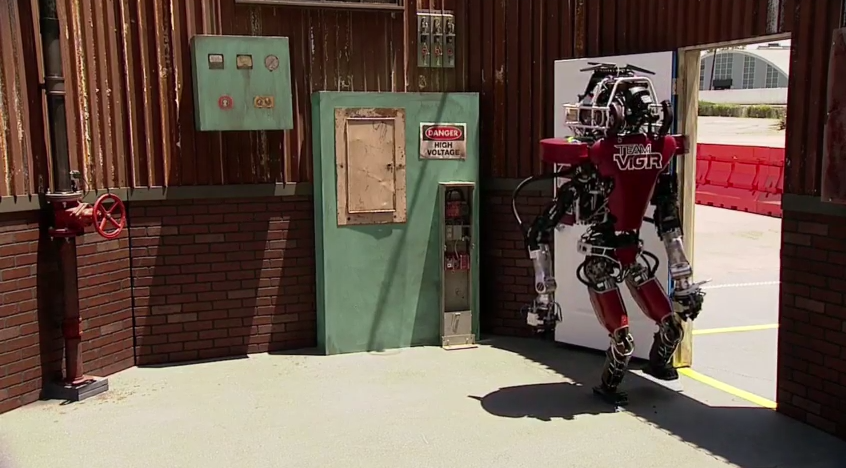
\includegraphics[width=0.99\columnwidth,clip]{./img/atlas_door_finals.png}
\caption{Team ViGIR's Atlas humanoid robot on the first day of the DRC Finals. (Photo credit: DARPA)
}
\label{Fig:AtlasDoorFinals}
\end{figure}

\begin{myExample}\label{Ex:PickupObject}
	Consider the high-level task: ``Walk to the valve and turn it" (Fig. \ref{Fig:AtlasDoorFinals}).
	This would be an intuitive way to express the task from a non-expert user's point-of-view.
	However, \ldots (not formal, preconditions, templates, reaction to failures, etc.)
\end{myExample}

\subsubsection*{Contributions (brain dump)}
\begin{itemize}
	\item Partial to full specification
	\begin{itemize}
		\item Most intuitive from the user�s point-of-view
		\item Limited message size over bad comms (send partial specification $\rightarrow$ compile and synthesize onboard)
	\end{itemize}	
	\item Multi-paradigm specification (objectives and initial conditions from user, topology/modes, preconditions, task)
	\todo[inline, caption = {Consider mutex for grounding conflicts in this paper?}]{Also consider mutex for grounding conflicts?}
	\item Generalization of activation--completion paradigm \cite{Vasu2013ICRA} Formalize how we deal with failures (and other outcomes). Graceful degradation. Human operators also included in environment.
	\item Integration with FlexBE and ROS
	\item Experimental validation on Atlas
\end{itemize}

\subsubsection*{Literature Survey}
\begin{itemize}
	\item Vasu's ``fast-slow" paradigm \cite{Vasu2013ICRA}
	\item Alternatives to LTL and GR(1) Synthesis
	\begin{itemize}
		\item Classic AI planners, STRIPS-type planners
		\item Optimization-based LTL synthesis (Eric Wolff)
		\item \textbf{co-safe LTL} (Lydia Kavraki, Calin Belta, etc.) We \emph{could} have used it as a different formalism and generated FlexBE state machines that way.
		\todo[inline, caption = {Comparison of GR(1) to co-safe LTL}]{Check whether co-safe LTL encodes reactivity w.r.t. adversarial environment (worst case)}
	\end{itemize}
\end{itemize}

%END